\documentclass[draft,linenumbers]{agujournal2018}
\usepackage{apacite}
\usepackage{url} % should fix any errors with URLs in refs.
\usepackage{amsmath}
%\usepackage{xcolor}
%\usepackage[colorlinks]{hyperref}
%\usepackage[colorinlistoftodos]{todonotes}

\draftfalse

\journalname{Space Weather}

\begin{document}

\title{Title}

\authors{R.S. Weigel\affil{1} and P.J. Cilliers\affil{2}}

\affiliation{1}{Space Weather Lab, George Mason University}
\affiliation{2}{South African National Space Agency}

\affiliation{1}{4400 University Drive, Fairfax VA 22030}
\affiliation{2}{Hospital Street, Hermanus 7200}

\correspondingauthor{R.S. Weigel}{rweigel@gmu.edu}

\begin{keypoints}
\item 
\item 
\item 
\end{keypoints}

\begin{abstract}
\end{abstract}

\section{Introduction}

\section{Data}
\label{section:Data}

\section{Models and Methods}
\label{section:Models_and_Methods}

To determine the coefficients $a_o$ and $b_o$ in the frequency independent model, Model~1,

\begin{linenomath*}
  \begin{equation}
    G_o(t) = a_oE_x(t) + b_oE_y(t)
    \label{model1}
  \end{equation}
\end{linenomath*}

\noindent

\section{Model Evaluation}
\label{section:Model_Evaluation}

\section{Results}
\label{Results}

\section{Discussion}
\label{Discussion}

\section{Conclusions}

\begin{figure}[h]
  \centering
  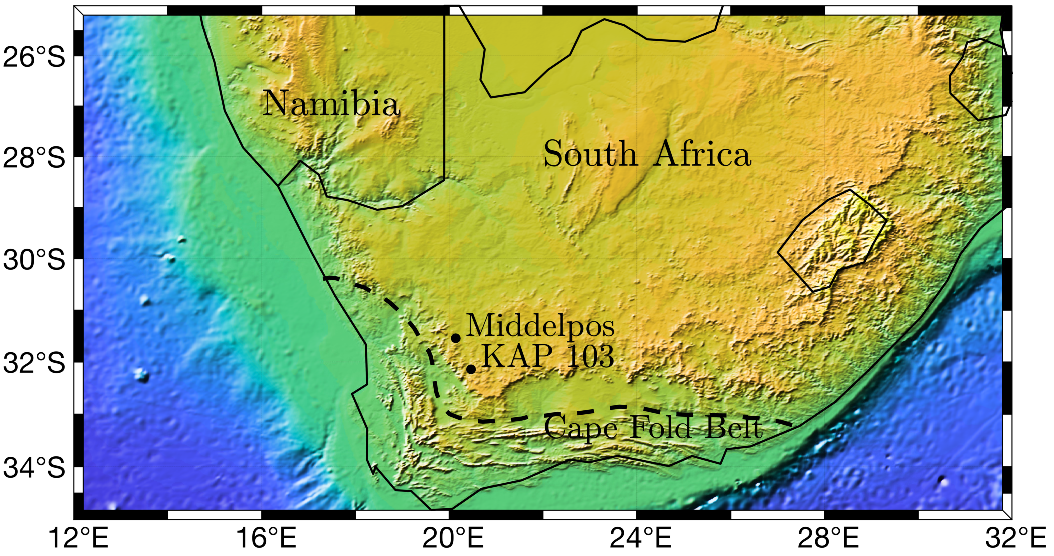
\includegraphics[width=\textwidth]{figures/map.pdf}
  \caption{Locations of measurement sites for GIC, at the Memanbetsu substation, and the geoelectric and geomagnetic field measurement site at Memanbetsu Magnetic Observatory. The red line corresponds to the path of the 187 kV power line. The distance from the observatory to the Memanbetsu substation is $\sim$9 km and dotted lines are Apex geomagnetic latitudes \citep{Richmond1995} in 2015.}
  \label{map}
\end{figure}

\clearpage

\section{Appendix}

\begin{table}
  \caption{Periods associated with evaluation frequency bands used for regression and smoothing spectra. \# is the evaluation frequency number, $N$ is the number of DFT points in the band, and $T_e\equiv 1/f_e$. The band range is from $T_l$ through $T_h$.}
  \centering
  \begin{tabular}{l l l l l}
    \hline \\
    \# & $N$ & $T_e$ [s] & $T_l$ [s] & $T_h$ [s] \\
    \hline \\
    1 & 2 & 43200 & 28800 & 86400 \\
    2 & 2 & 28800 & 21600 & 43200 \\
    3 & 3 & 21600 & 14400 & 43200 \\
    4 & 4 & 14400 & 9600 & 28800 \\
    5 & 5 & 10800 & 7200 & 21600 \\
    6 & 6 & 7854.5 & 5400 & 14400 \\
    7 & 8 & 5760 & 3927.3 & 10800 \\
    8 & 12 & 3927.3 & 2618.2 & 7854.5 \\
    9 & 16 & 2880 & 1920 & 5760 \\
    10 & 22 & 2009.3 & 1350 & 3927.3 \\
    11 & 31 & 1440 & 960 & 2880 \\
    12 & 43 & 1016.5 & 680.3 & 2009.3 \\
    13 & 61 & 720 & 480 & 1440 \\
    14 & 85 & 511.2 & 341.5 & 1016.5 \\
    15 & 120 & 361.5 & 241.3 & 720 \\
    16 & 170 & 255.6 & 170.4 & 511.2 \\
    17 & 240 & 180.8 & 120.5 & 361.5 \\
    18 & 338 & 128 & 85.4 & 255.6 \\
    19 & 478 & 90.5 & 60.3 & 180.8 \\
    20 & 676 & 64 & 42.7 & 128 \\
    21 & 956 & 45.2 & 30.2 & 90.5 \\
    22 & 1351 & 32 & 21.3 & 64 \\
    23 & 1910 & 22.6 & 15.1 & 45.2 \\
    24 & 2701 & 16 & 10.7 & 32 \\
    25 & 3819 & 11.3 & 7.5 & 22.6 \\
    26 & 5401 & 8 & 5.3 & 16 \\
    27 & 7638 & 5.7 & 3.8 & 11.3 \\
    28 & 10801 & 4 & 2.7 & 8 \\
    \hline \\
  \end{tabular}
  \label{evaluationperiods}
\end{table}

\clearpage

\bibliography{paper.bib}

\end{document}
